\section{Method}
Here the methodology and equipment choices of the performed experiments are described. The logical place to begin is with the silicon chips, which are the central object of interest in the experiments. The chips used were had a typical area of \SI{1}{\centi\meter^2} and a thickness of a few millimetres. In order to couple light into the waveguides etched onto the chip spot size converters or diffraction gratings are used. For spot size converters figure \ref{coupling} shows the procedure. The fibre which directs the light is called a lense fiber, it has a focal point a few micrometers in front of its tip, allowing high accuracy coupling onto the converters. For this type of coupling peizometers were used with a recoupling algorithm. 
\newline

\begingroup
    \centering  
    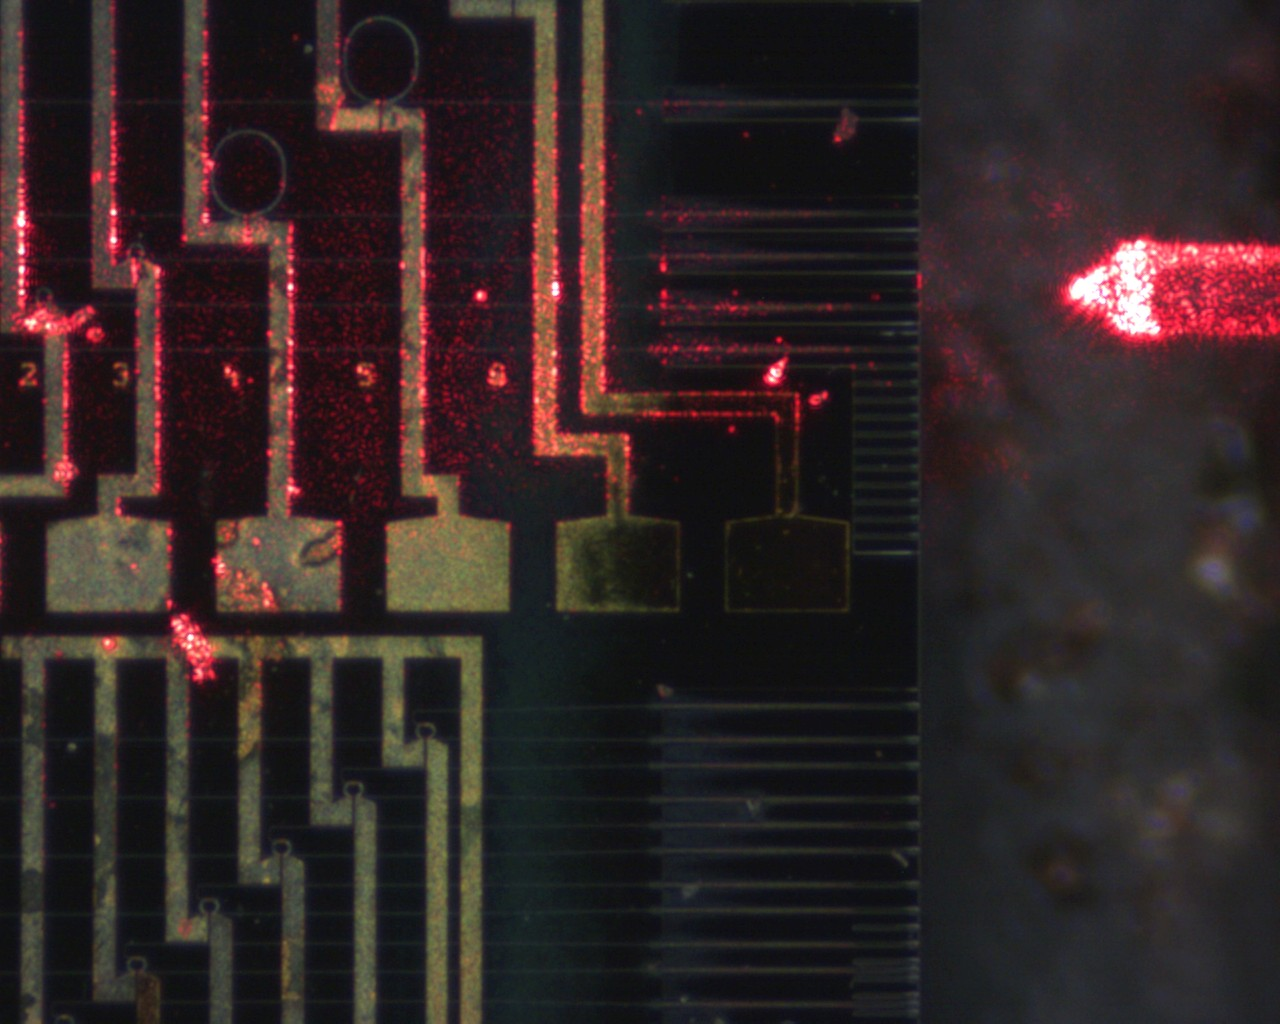
\includegraphics[width=5.3cm]{img/method/chipPictures/redLaser_aboveChip.jpg}
    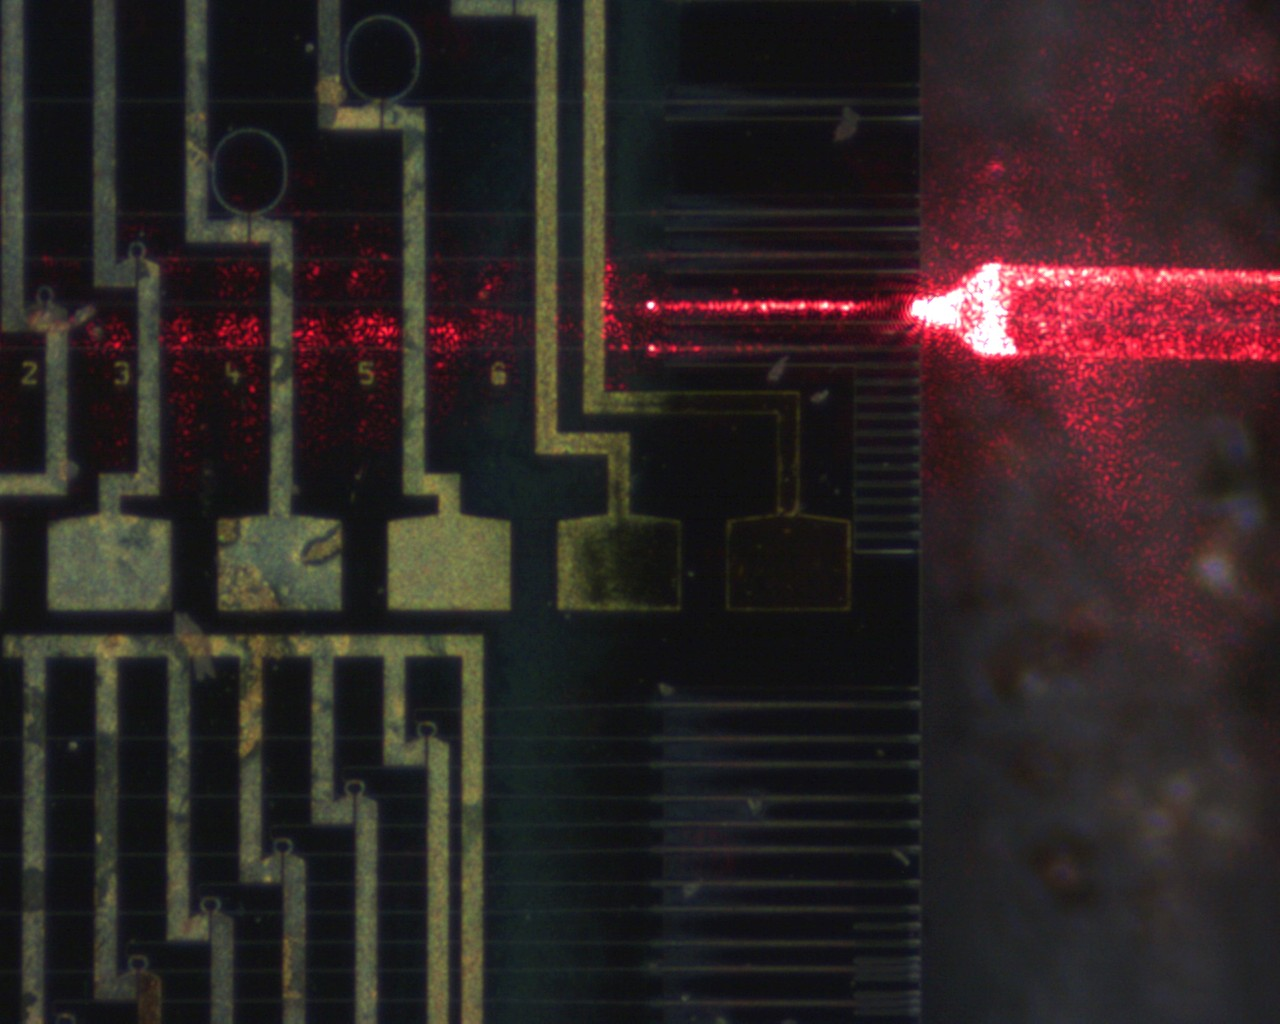
\includegraphics[width=5.3cm]{img/method/chipPictures/redLaser_coupled.jpg}
    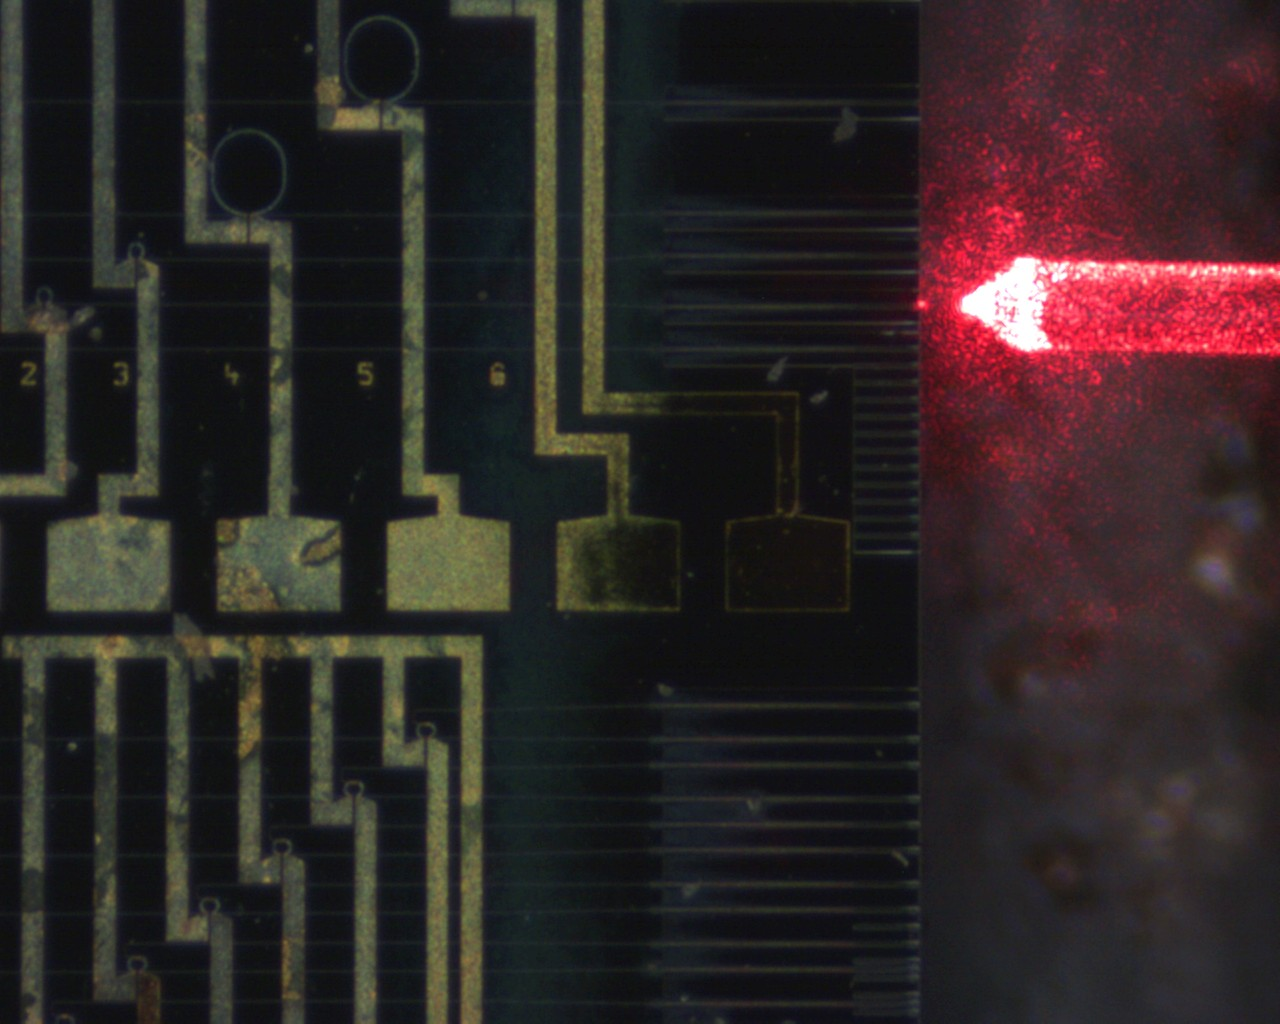
\includegraphics[width=5.3cm]{img/method/chipPictures/redLaser_belowChip.jpg}
    \captionof{figure}{The first image shows the lense fiber above the chip, illuminating its surface, then the fiber has found a good coupling position and finally it is too far underneath the chip. Red light is used for convenience and all other work is done with infared light.}
     \vspace{3pt} \label{sideCoupling}
\endgroup

The second way of getting light onto a chip is via diffraction gratings, these are small structures which couple light into a waveguide, figure \ref{verticalCoupling} shows this process from two views. Here the ideal coupling region is much larger, so there is no need for computer control and manual adjustment can suffice.
\newline

\begingroup
    \centering  
    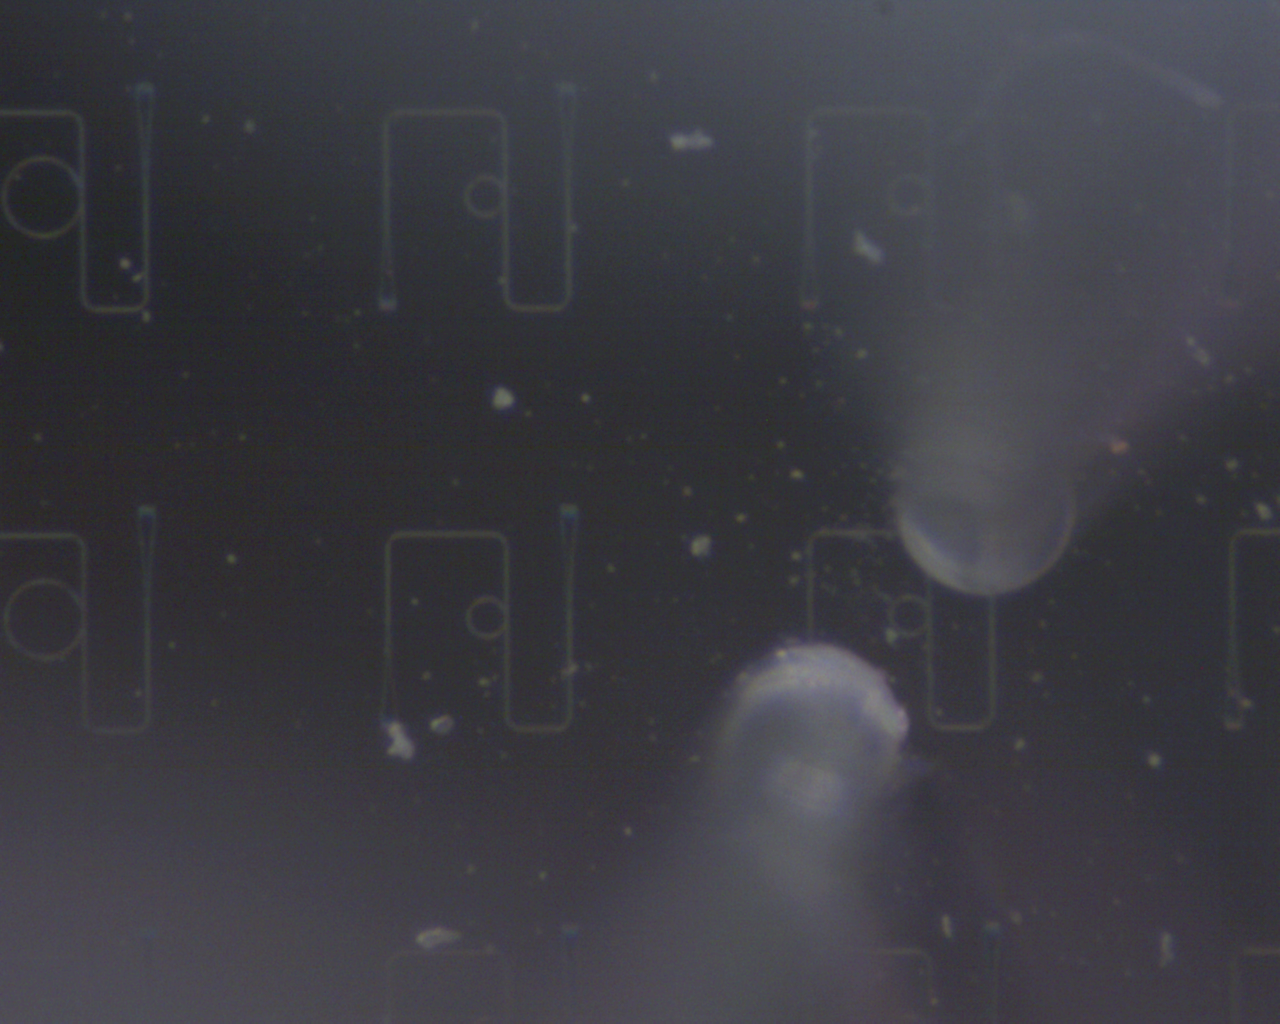
\includegraphics[width=7cm]{img/method/chipPictures/verticalCouplingTopView.png}
    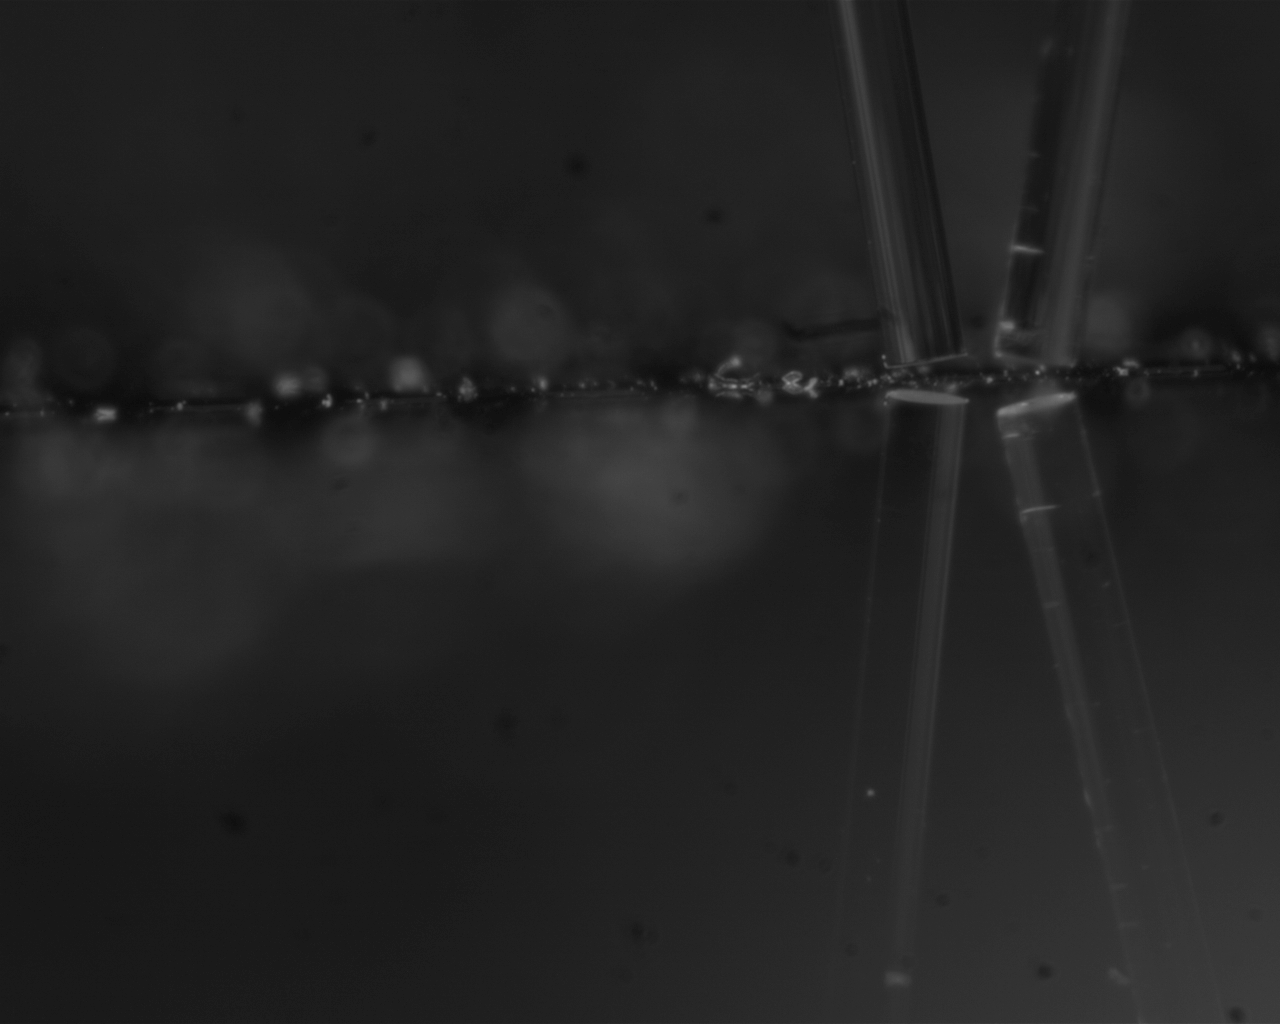
\includegraphics[width=7cm]{img/method/chipPictures/verticalCouplingSideView.png}
    \captionof{figure}{Side coupling proceedure}
     \vspace{3pt} \label{verticalCoupling}
\endgroup

All of these coupling techniques rely on powermeters in the infrared region to maximise the transmission through the chip. Further the polarisation of the light must be adjusted to be inline with the mode which the devices is designed for. 

With light reliably coupled into the chip a spectral scan of the wavelength range \SI{1530}{\nano\meter}-\SI{1560}{\nano\meter} is typically performed to get a transmission spectra like in figure \ref{ringResTrans}. With this the quality factor and the coupling coefficients of the particular ring can be calculated. 

To begin the process for collecting a joint spectrum, the set up is arranged as in figure \ref{simpleJSI}. This maintains the ability to do the above initial procedure. The two power meters allow the loss due to coupling to be monitored. This is typically on the order of \SI{20}{\deci\bel\m}.

\begingroup
    \centering  
    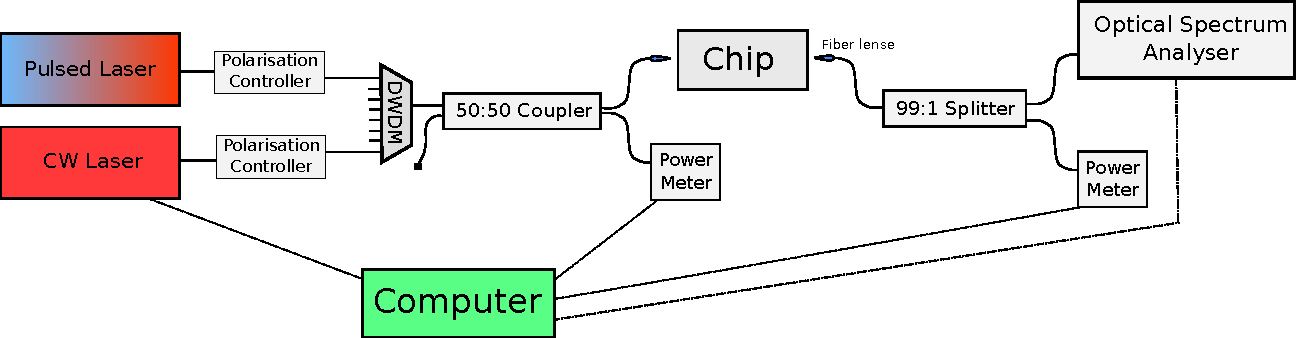
\includegraphics[width=18cm]{img/method/setup_1.pdf}
    \captionof{figure}{Glassgow test structure chip}
     \vspace{3pt} \label{simpleJSI}
\endgroup

The wavelength division multiplexer (DWDM) has 16 channels with \SI{90}{\deci\bel\m} noise suppression. These are used to suppress the amplified spontaneous emission (ASE) both lasers produce. With temperature control of the chip the resonances are tuned to the center of the DWDM channels. Then two resonances are chosen, onto one the pump is tuned and the other is connected to the CW laser in prepration for the stimulated four wave mixing. 

Figure \ref{aSiBigPicture} is a key illustration of this experiment. One difference here is that the CW laser is instead filtered by a tunable filter as in figure \ref{bigJSIExp} so the limits of the channel are not present. These are typically on the order of \SI{1}{\nano\m}.

\begingroup
    \centering  
    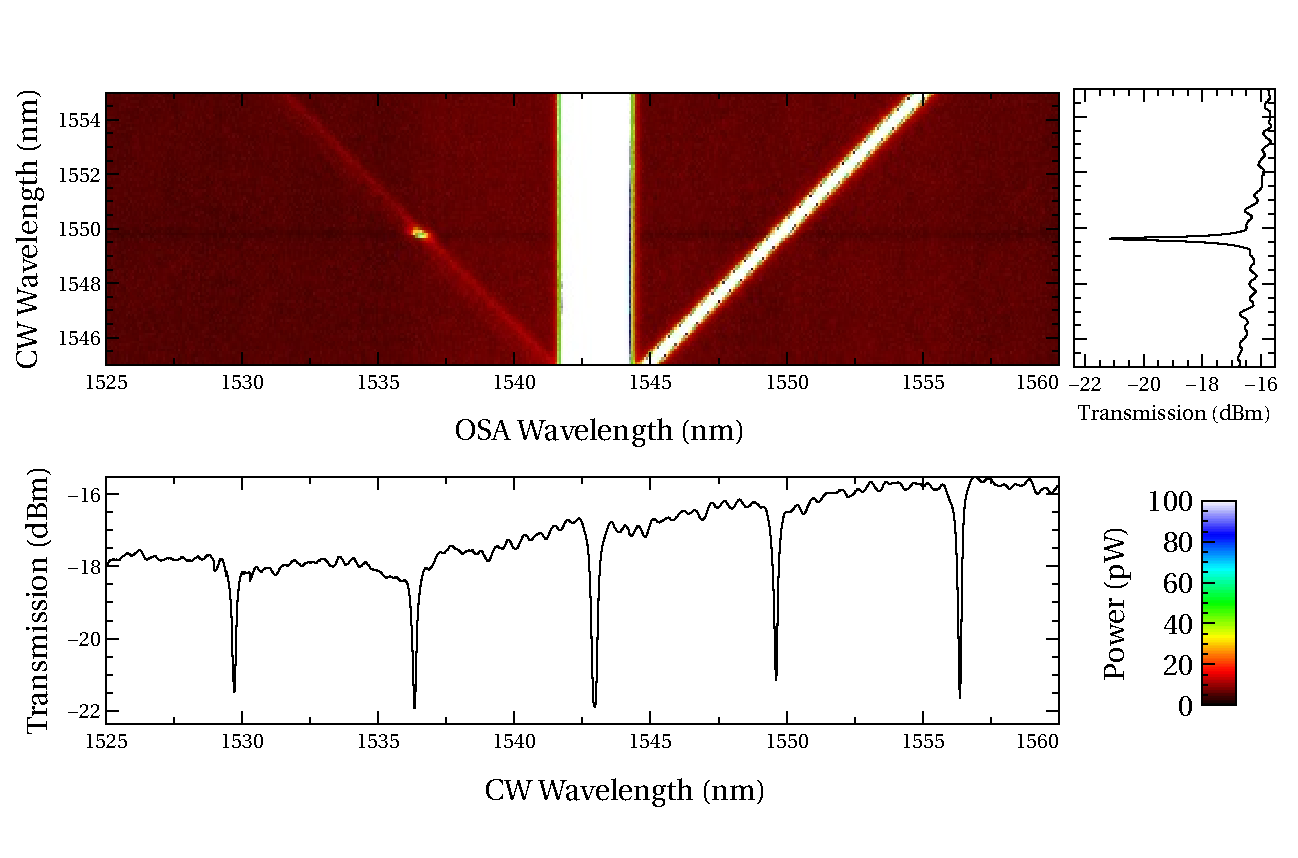
\includegraphics[width=18cm]{img/method/aSiBigPicture.pdf}
    \captionof{figure}{big picture}
     \vspace{3pt} \label{aSiBigPicture}
\endgroup



\begin{itemize}
	\item {\bf Glassgow }
	\item {\bf Toshiba }
	\item {\bf HP }
\end{itemize}

\begingroup
    \centering  
    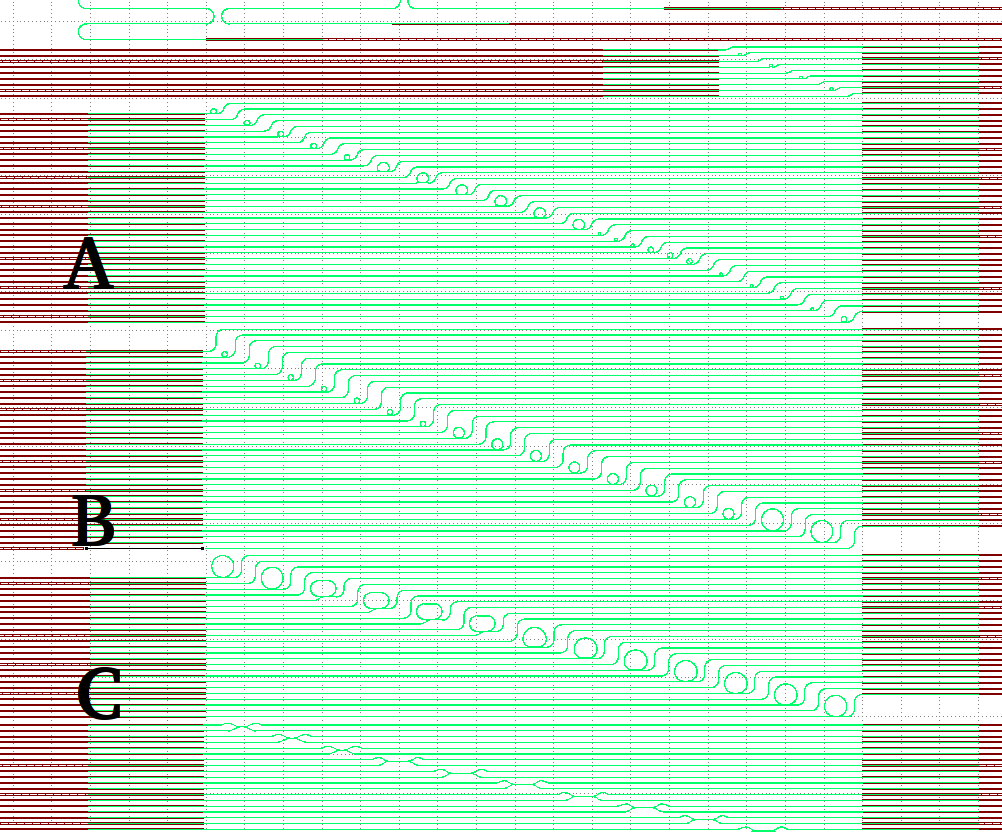
\includegraphics[width=10cm]{img/method/glassgowChipNumbering.png}
    \captionof{figure}{Glassgow test structure chip}
     \vspace{3pt} \label{crossCompare}
\endgroup

\begingroup
    \centering  
    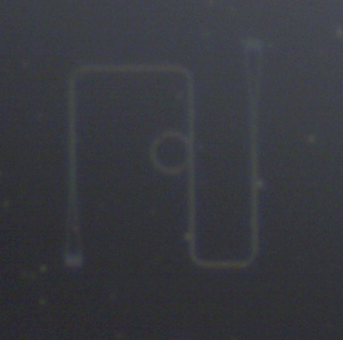
\includegraphics[width=10cm]{img/method/chipPictures/exampleASIRing.png}
    \captionof{figure}{Glassgow test structure chip}
     \vspace{3pt} \label{crossCompare}
\endgroup


\begingroup
    \centering  
    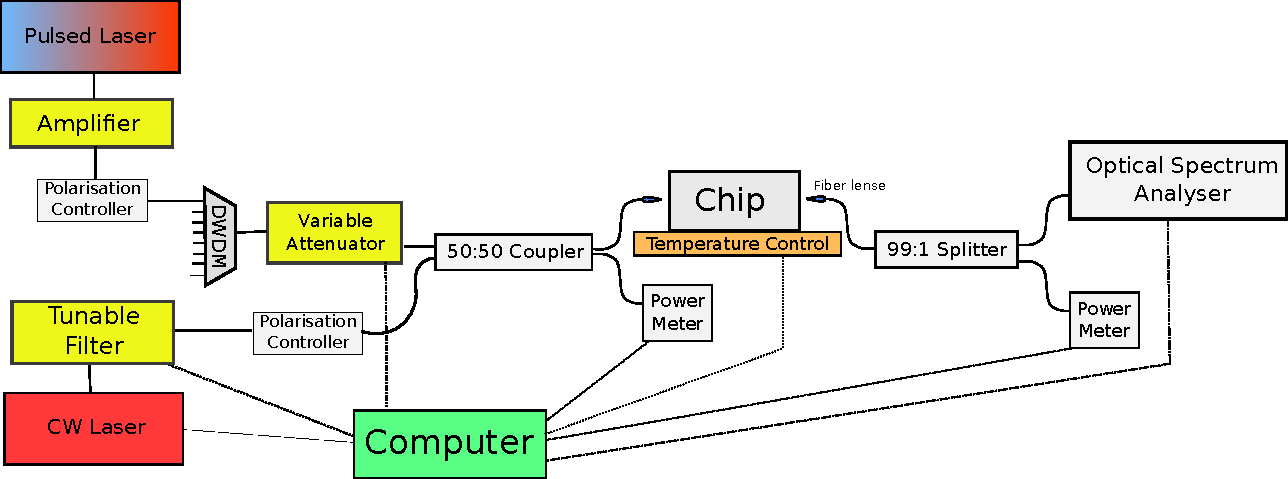
\includegraphics[width=18cm]{img/method/setup_2.pdf}
    \captionof{figure}{big experiment}
     \vspace{3pt} \label{bigJSIExp}
\endgroup
\begingroup
    \centering  
    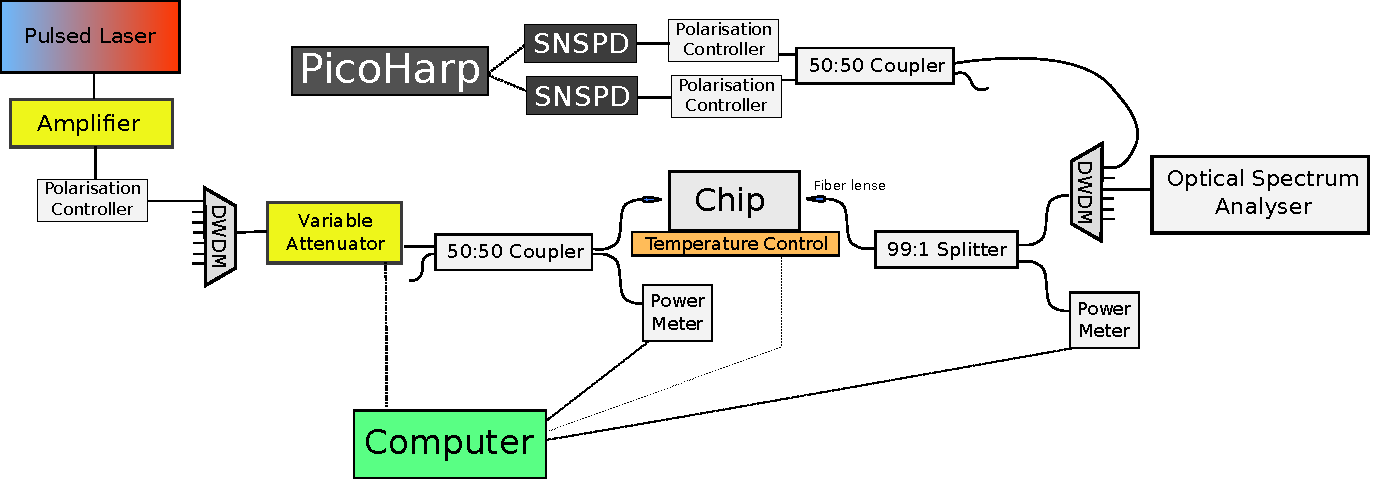
\includegraphics[width=18cm]{img/method/setup_3.pdf}
    \captionof{figure}{single photon}
     \vspace{3pt} \label{crossCompare}
\endgroup

% Side/Vertical coupling
% Coupling loss
% Blowing up chips -> tempted to add this as a complaint
%	Particularly on glassgow chip
% Temperature tuning



\subsection{Joint Spectrum}
Take the convention that the {\bf signal} photon is the one we measure and the {\bf idler} is the one we stimulate.
% OSA Resolution discussion might be important. Because I think it might have skrewed me over somewhat.
% Filtering
% Could reference the model so that I don't have to use example data.
\subsection{$g^{(2)}(0)$}
% Breif description of how this works.
\subsection{Analysing Data}
% The algortihm reflects how using narrow filters increases the purity well
% SNR
% NOISE
% NORALISATION
% SPM
% RING DEFORMATION
% How to calculate Q, r, tau
% Comparing with the simulation

% I want to really discuss what we can hope to keep constant and what we can vary. Where you need to really do som engineering to get insights.